% !TEX root = ./tech-specification.tex

%%%%%%%%%%%%%%%%%%%%%%%%%%%%%%%%%%%%%%%%

\section{Consensus}

The consensus rules in {\name} are designed to make decision on two questions: the first is that whether a block is valid and should be added to the {\name} blockchain; the other is that in what order those valid blocks should be processed.   

In an overview, the \name consensus protocol optimistically accepts all formally correct blocks and organizes them as a \tg (instead of a tree or a chain), and then specifies a total order of blocks in the \tg following the \oldversion{Conflux consensus rules in \cite{Conflux}} \newversion{GHAST rule}.
This total order will be agreed by all honest participants and it is hard to change (under reasonable assumptions). 
After fixing such an order, transactions inside blocks are executed accordingly, and invalid transactions, which can be duplicating or conflicting previously processed transactions, are ignored.

% \newversion{
% 	We remark that the referee validation only  validates the parent edge choice with in its EraGenesis subtree.
% }


\subsection{Validation of Blocks}
\label{sec:block validate}

A set of {\name} blocks form a \tg structure where each vertex in the \tg represents a {\name} block and each directed edge in the \tg corresponds to a parent or referee reference. 
Every full node maintains a \tg structure of accepted blocks, which are blocks that are valid in the node's local view.
Whenever receiving a new block, the full node verifies whether the block is valid before adding it into the \tg.

The validation of a new block can result in four outcomes:
\begin{itemize}
	\newversion{\item {\bf suspending:} the block $\block$ is partially valid and $\timerdis(\block;\graph)< \pbeta$. ($\timerdis(\cdot)$ is defined later in eq.~(\ref{def:timerdis}) and $\graph$ denotes the current \tg.) 
	The status of block $\block$ will be checked again each time a new valid (or partially valid) block appears in the future set of $\block$. }

	\item {\bf accept:} the block is valid \newversion{(either fully valid or partially valid but not \textbf{suspending} anymore)} and will be added to the \tg immediately.
	      
	\item {\bf reject:} the block is clearly invalid and will be discarded.
	      
	\item {\bf pending:} the block references some blocks not in the current \tg. Such blocks will be checked again once all the referenced blocks have been added to the \tg.
\end{itemize}
%
\medskip
Given a new block $\block$ that is no longer {\bf suspending}, the validation of $\block$ is done in the following steps:
\begin{enumerate}[]
	\item {\bf Header Validation.} This step asserts that $\block$ has a valid header (or at least a partially valid one) following Section~\ref{sec:valid header} and \ref{sec:pvalid header}.
	      Note that a {\bf Proof-of-Work Validation} of $\block$ is embedded inside the {\bf Header Validation},
	      where the solution to the $\pow$ puzzle is verified w.r.t. the legitimate target difficulty $\head(\block)_{d}$. 
	      The canonical gas limit $\head(\block)_{\ell}$ is also checked here, i.e. $\head(\block)_{\ell}\in \left(1\pm \frac{1}{1024}\right)\times \head(\parent{\block})_{\ell}$ and $\head(\block)_{\ell}\ge \mingaslimit$ as in (\ref{eq:blockgas}).
	      
	      The {\bf Proof-of-Work Validation} is the major mechanism against Sybil attacks and should be performed before invoking more expensive steps of verification and execution.
	      It is interchangeable with 
	      other steps of the validation for better efficiency;
	      % the {\bf Referee Validation}, especially in case when there are too many pending blocks;
	      and it will be performed last and repeatedly when mining a new block.
	      
	      
	\item {\bf Referee Validation.} The validation of referee headers asserts that $\block$ only references existing valid blocks. 
	      % \guangsays{Shall we put an upper bound for the number of referee references in each block?}
	      In case the new block references the head of an unknown block, it is marked as {\bf pending} until all its referee blocks have been added to the \tg.
	      The node is suggested (but not forced) to query its neighbors about the referenced unknown block.
	      	
	      		      
	
	\item {\bf Volume Validtion.} The size of block body must not exceed \maxblocksize. 
	Formally, $\sum_{\tx\in\block_\txs} \left| \rlp(\tx)\right| \le \maxblocksizeinbytes$.

	      
	\item {\bf Internal Consistency.} This step asserts that $\block$ is self-consistent.
	      More specifically:
	      \begin{itemize}[nosep]
	      	\item the block header $\block_\head$ is formally consistent with content in $\block_\txs$,
	      	      i.e. $\block_\head$ is well-formed following Section~\ref{sec:internal consistency};
	      	      
	      	\item every transaction $\tx\in\block_\txs$ is \emph{locally legitimate}, 
	      	      which is the first test of the intrinsic validity of transactions:
	      	      \begin{enumerate}[nosep]
	      	      	\item $\tx$ is well-formed $\rlp$ with no trailing bytes; 
	      	      	      
	      	      	\item $\tx$ has a valid signature by its sender $\sender{\tx}$;

  	      	      	% \item $\tx$ has a valid recipient, i.e. the type indicator (first $4$-bit) of $\tx_a$ belongs to $\set{\typereserved,\typenormal,\typecontract}$;

	      	      	\item $\tx$ has correct chain id $\tx_c = \chainid$;
					
					\item the \textbf{gasLimit} $\tx_g$ is no smaller than the intrinsic gas $g_0$, where
					\begin{align}\label{def:g0}
						g_0\eqdef 
						&\sum_{i\in \tx_{\bf i}, \tx_{\bf d}} \begin{cases}
							G_\mathsf{txdatazero} & \mbox{if $i=0$}\\
							G_\mathsf{txdatanonzero} & \mbox{otherwise}
						\end{cases}\notag\\
						&+ \begin{cases}
							G_\mathsf{txcreate} & \mbox{if $T_a=\emptyset$}\\
							0 & \mbox{otherwise}
						\end{cases}\notag\\
						&+ G_\mathsf{transaction}
					\end{align}
	      	      \end{enumerate}
	      	      
	      	\item the total gas consumption does not exceed the block gas limit, i.e. $\sum_{\tx\in \block_{\txs}} \tx_g \le \block_{\head_{\ell}}$.
	      	      % 
	      	      % \item \guangsays{anything else?}
	      \end{itemize}
	      
	      	
	      
	\item If $\block$ passes all above steps, then it is marked {\bf accept} and added into the \tg structure, otherwise it is marked {\bf reject} and discarded.
\end{enumerate}

Note that because a valid block must pass all the above validation steps and there is no jump or loop, 
all validation steps are interchangeable and parallelizable. 


We emphasize an important difference of {\name} from other blockchains in validating blocks: 
in {\name} we check the validity of each transaction locally,
i.e. at this moment we do not care if it is a duplicate of some processed transaction or the sender has insufficient balance.
Thus a block $\block$ being valid \textbf{does not} imply that all transactions in $\block_\txs$ are valid or will be eventually executed.
The validation of transactions in $\block_\txs$ will be deferred to the finalization of $\block$.



\subsection{Total Order in the \tg}


Every {\name} full node maintains a \tg structure of accepted blocks, and now we discuss how to decide the total order of all accepted blocks.

Recall that in the \tg each vertex represents a {\name} block and each directed edge represents the reference of another block.
The vertex for the genesis block has no outgoing edges, since the genesis block does not reference any other block.
Other than the genesis block, each block has exactly one parent reference and possibly multiple (can be zero) referee references, represented by multiple outgoing edges from the corresponding vertex.
This directed graph is acyclic since every directed edge reflects a clear chronological order of blocks, unless the referenced block is generated using a hash collision. 
% Furthermore, if we only consider parent edges, the blocks would form a tree structure, on which we will first define the pivot chain based on the GHOST rule \cite{GHOST} 
Based on this \tg structure the {\name} consensus will first select a pivot chain that defines order of blocks on the chain, and then extend to the total order of all blocks. 


\newversion{
	\subsubsection{GHAST and Weight Adaption on the \tg}
	\label{subsec:GHAST}

	In {\name} the valid blocks may have heterogeneous weights, even if there is no difficulty adjustment.
	This feature is introduced to improve the liveness guarantee in case a divergence of computing power (which is also the block generation power) happens, either by chance or caused by an active attack.

	At a high level, the GHAST rule defines block weight as follows:
	\begin{itemize}
		\item In the usual case,  all valid blocks have homogeneous weight. 
		That is, every block with a proof of work satisfying the target difficulty of the epoch it belongs to would have the same weight, say weight $1$.	

		\item When a divergence of block generation power is observed, the distribution of block weights is changed adaptively:

		\begin{itemize}
			\item A small fraction of blocks are marked as ``heavy blocks'' and given a greater weight.
			In particular, if the attached proof of work of a block has difficulty at least $\heavywvalue$ times of the epoch's normal target difficulty, then this block is called a \emph{heavy block} and its weight is also $\heavywvalue$ times of a usual block, so as its base award.

			\item Other blocks under this circumstance are still valid as long as the attached proof of work satisfies the normal target difficulty. But they have zero weight when making consensus decisions.

			\item When the divergence is resolved, the weight distribution resumes to the usual case, where every block with a valid proof of work has the same weight as target difficulty of the epoch.
		\end{itemize}	
	\end{itemize}

	To be more specific,
	we remark that the GHAST rule only considers blocks in recent eras, e.g. the choice of parent edge is defined and validated \emph{within} the subtree of the corresponding era genesis.
	See Section~\ref{sec:checkpoint} for more details about era and checkpoints.


	\paragraph{Timer Chain}
	\label{sec:timer chain}

	\name introduces the notion of timer block and timer chain as a robust estimation of elapsed time.
	Intuitively the timer chain is the longest chain that would be generated if the block generation were slow, or equivalently only high quality blocks were considered.

	Every \textbf{fully valid} block $\block$ with quality $\quality(\block)\ge \timerweight\cdot \block_d$ is called a \emph{timer block}.
	The partial order of timer blocks can be deduced from the \tg of all blocks,
	which then determines the longest chain of timer blocks, called the \emph{timer chain}.	
	More specifically, the genesis block is also genesis of the timer chain, and the ``parent timer block'' of every timer block $\block$ is recursively defined by choosing the tip of timer chain in $\past(\block)$. 
	For convenience, the parent timer block of $\block$ is denoted by $\parentf_{timer}(\block)$.

	For convenience the timer chain in \tg $\graph$ is denoted by $\timerchain(\graph)$,
	and the difference of timer blocks in two {\tg}s $\graph$ and $\graph'$ is denoted by $\timerdis(\graph,\graph')$ as follows
	\begin{align}\label{def:timerdis}
		\timerdis(\graph,\graph') \eqdef \left|\timerchain(\graph) 
		\backslash  \graph' \right|
	\end{align}
	The timer block difference $\timerdis(\graph,\graph')$ provides an estimate of the time difference between two local views $\graph$ and $\graph'$.




	\paragraph{Triggering Condition of Adaptive Weight}
		

	Intuitively, a block $\block$ should apply the adaptive weight rule if any previous pivot block (on $\chain(\block)$) fails to 
	receive support from a clear majority of computing power,
	i.e. the nemesis pivot block does not accumulate enough weight under its subtree after a sufficiently long time.
	
	Formally, 
	a block $\block$ is an \emph{adaptive block}, denoted by $\mathrm{Adaptive}(\block)=\true$,
	if there exists $\block'\in\chain(\block)$ satisfying both of the following conditions:
	\begin{enumerate}[]
		\item $\timerdis\left(\past(\block),\past\left(\parentf(\block')\right) \right)\ge \pbeta$;

		\item $\mathsf{SubTW}\left(\block';\past(\block)\right) - \left( \mathsf{SubTW}\left(\parentf(\block');\past(\block)\right)-\mathsf{SubTW}\left(\block';\past(\block)\right)-\weight\left(\parentf(\block')\right)\right) < \palpha \cdot \block_d$,

		where $\mathsf{SubTW}(\ablock;\graph)$ denotes the total weight of the sub-tree rooted at $\ablock$ in graph $\graph$,
		and $\weight(\cdot)$ is the adaptive weight function as defined in (\ref{def:weight}).
	\end{enumerate}


	Otherwise the block $\block$ is a \emph{non-adaptive block} and denoted by $\mathrm{Adaptive}(\block)=\false$. 
	%
	The adaptive weight mechanism is only triggered for adaptive blocks.


	


	\paragraph{Adaptive Block Weight}
	% \label{subsec:AdaptiveWeight}

	Recalling that $\pow(\cdot)$ denotes the proof-of-work function  and $\block_d$ denotes the target difficulty of $\block$, 
	the GHAST rule formally defines the weight of a block $\block$ as follows:
	\begin{align}\label{def:weight}
		\weight(\block) \eqdef 
		\begin{cases}
		\block_d       & \text{if } \neg\; \mathrm{Adaptive}(\block)                                 \\
		0       & \text{if } \mathrm{Adaptive}(\block) \;\land\; \heavywvalue \cdot \pow(\block_\head) \cdot \block_d > {2^{256}} \text{ (i.e. $\quality(\block) < \heavywvalue  \cdot \block_d$)} \\
		\heavywvalue\cdot \block_d & \text{if } \mathrm{Adaptive}(\block) \;\land\; \heavywvalue \cdot \pow(\block_\head) \cdot \block_d  \le  {2^{256}} \text{ (i.e. $\quality(\block) \ge \heavywvalue  \cdot \block_d$)}   
		\end{cases} 
	\end{align}   


	We remark that whether a block $\block$ should be adaptive or not is fully determined by $\past(\block)$, which is indeed specified by $\block$ through directly and indirectly referenced blocks.
	Therefore it is not necessary to put a specific flag in the header of $\block$ for this condition, unless for efficiency concerns. 
}


\subsubsection{\newversion{The GHAST Rule} for Selecting the Pivot Chain }
\label{subsec:GHAST parent}

Since every block (except the genesis block) has exactly one parent, all parent edges in the \tg together form a \emph{parental tree} with the genesis block being the root. 
In the parental tree, {\name} \newversion{applies the GHAST rule} to select a chain from the genesis block to one of the leaf blocks as the \emph{pivot
chain},
where blocks on the pivot chain are called \emph{pivot blocks} and other blocks called \emph{off-pivot blocks}.

In {\name} the pivot chain is not necessarily the longest chain or the ``heaviest'' chain.
\newversion{Indeed, the GHAST rule requires that the pivot chain should proceed to the branch whose subtree has greatest total weight (after weight adaption), in case there are multiple child blocks to choose}. 
% 
The {\name} selection algorithm starts from the genesis block. 
At each step, it computes the accumulated 
\newversion{\emph{total weight}} of each child subtree in the parental tree and advances to the child
block whose subtree has the largest total \newversion{weight}, until it reaches a leaf block in the local \tg. 

The total \newversion{weight} of a subtree rooted at block $\block$ is denoted by $\block_t$ and defined recursively as:
\begin{align}
	\block_t \eqdef \block_d + \sum_{\block': \parent{\block'}=\block} \block'_t 
	% \begin{cases}                                                                          
	% 	\head_d & \mbox{if $\block$ is a leaf block}                                                                          \\
	% 	\head_d + \sum_{\block': P(\block')=\block} \block'_t & \mbox{otherwise}                                                                          
	% \end{cases}                                                                          
\end{align}
where $\block_d\eqdef \head(\block)_d$ denotes the target difficulty of $\block$, 
and $\parent{\block'}$ is the parent block of $\block'$ (hence the summation is taken over $\block$'s children).
Note that $\block_t$ is not a part of the block $\block$ -- indeed it describes a state of $\block$ in the local view and may increase as more subsequent blocks are included afterwards.

We further remark that the total \newversion{weight} of every subtree can be computed from all block headers, 
since a block header contains the block difficulty as well as its parent \newversion{and referees}, which suffices to decide \newversion{the weight of this block as in Section~\ref{subsec:GHAST} and hence} the total \newversion{subtree weight} recursively.
As a result, the whole pivot chain can be determined by the block headers.


The advantage of \newversion{the GHAST rule} is that it guarantees the
irreversibility of the selected pivot chain even if honest nodes fork because of network delays or other reasons.
This is because forked blocks also contribute
to the safety of the pivot chain (indeed, this property is inherited from GHOST rule, c.f.~\cite{GHOST}).

For example, consider the local view as in Figure~\ref{fig:example} and for simplicity suppose that all blocks have equal weight. 
{\name} would select \phvname{Genesis}, \phvname{A},
\phvname{C}, \phvname{E}, and \phvname{H} as pivot blocks. 
Note that they do not form the longest chain in the parental tree -- the longest chain is
\phvname{Genesis}, \phvname{B}, \phvname{F}, \phvname{J}, \phvname{I}, and \phvname{K}. 
{\name} does not select that longest chain because the subtree of
\phvname{A} contains more blocks (and hence more total amount of computation) than the subtree of \phvname{B}. 
Therefore, the chain selection algorithm selects \phvname{A} over \phvname{B} at its first step.

\begin{figure*}
	\centering
	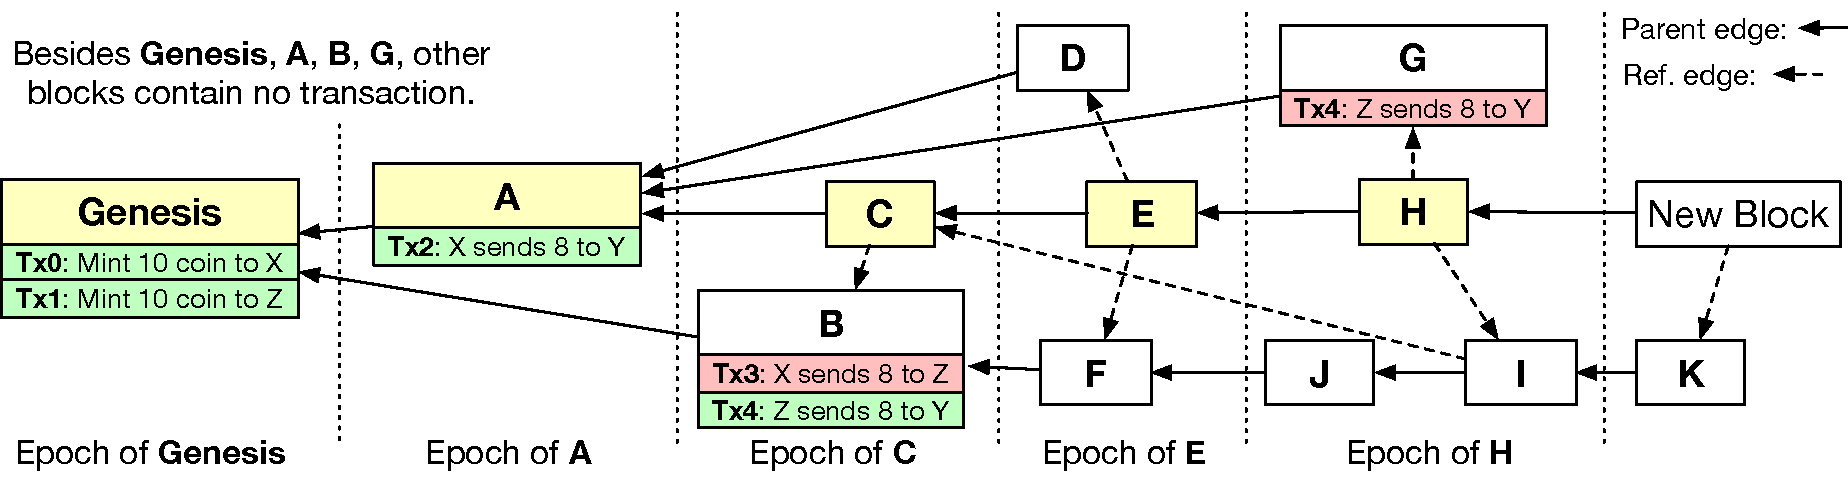
\includegraphics[scale=0.52]{figs/example}
	\caption{An example local \tg state to illustrate the consensus algorithm of
		{\name}. The yellow blocks are on the pivot chain in the \tg. 
		Each block on the pivot chain forms a new epoch to partition
		blocks in the \tg.}
	\label{fig:example}
\end{figure*}




\subsubsection{Epoch}

Given the pivot chain in a \tg,  {\name} splits all blocks into epochs as follows:
\begin{itemize}[nosep]
	\item Every pivot block $\block$ is at epoch $\head(\block)_h$, or simply the \emph{epoch of} $\block$, which is denoted by $\epf(\block)$.
	In particular the genesis block is at epoch $0$.
	      
	\item Every off-pivot block $\block'$ is at the epoch of the first pivot block $\block$ that references it, directly or indirectly. 
	That is, every block $\block'\in \referees(\block)$ is at the epoch of $\block$; then every block $\block''$ referenced by $\block'$, i.e. $\block''\in \referees(\block')\union \set{\parent{\block'}}$, if not already included in an earlier epoch, is also at the epoch of $\block$; and recursively all blocks referenced by $\block''$ and so on.
\end{itemize}

In other words, the epoch of $\block$ consists of all blocks within the local view of $\block$, such that there blocks are potentially produced after $\parent{\block}$ but clearly before $\block$.
% 
For example, 
each of the pivot blocks \phvname{Genesis}, \phvname{A},
\phvname{C}, \phvname{E}, and \phvname{H} corresponds to one individual epoch in Figure~\ref{fig:example}. 
The block \phvname{J} belongs to the epoch of \phvname{H} but not the epoch of \phvname{E}, because \phvname{J} is
reachable from \phvname{H} but not reachable from the previous pivot block \phvname{E}.

It is clear from the definition that as long as the pivot chain is not reverted, the partition of epochs cannot be changed.

\newversion{
\paragraph{Epoch capacity}
	Each epoch now has a limit of executing $200$ blocks. When a single epoch contains more than $200$ blocks, {\name} will only execute the last $200$ blocks (as specified in Section~\ref{sec:total order}) in that epoch. 
	This limit is introduced to battle DoS attacks about releasing a lot of blocks suddenly.
}


\subsubsection{Total Order of Blocks}
\label{sec:total order}

{\name} extends the total order of pivot blocks to all blocks in a \tg as follows.
{\name} first sorts blocks according to their corresponding epochs, so that a block in an earlier epoch always precedes another block in a later epoch;
and then {\name} sorts the blocks inside each epoch based on their topological order, i.e. corresponding to the partial order implied by referee references.
In case two blocks have no partial order relation, {\name} breaks ties deterministically with the unique ids of these two blocks. 
{More detailed rules are described with codes in Figure~\ref{fig:order}.}

\begin{algorithm}[!htb]
	\small
	\SetNlSty{}{}{}
	\DontPrintSemicolon
	\SetKw{To}{ to }
	\SetKw{In}{ in }
	\SetKw{And}{ and }
	\SetKwInOut{Input}{Input}\SetKwInOut{Output}{Output}
	\Input{ A block $\block$ and the local \tg $\graph$ (with $\block$ in $\graph$ and $\gblock$ is the genesis block of $\graph$)}
	\Output{A list of blocks $\mathbf{L} = \block_1 \circ \block_2 \circ \ldots \circ \block_n$, where $\block_1,\dots, \block_n$ are blocks in $\graph$, and in particular $\block_1 = \gblock$ and $\block_n=\block$}
	\let\oldnl\nl% Store \nl in \oldnl
	\newcommand{\nonl}{\renewcommand{\nl}{\let\nl\oldnl}}% Remove line number for one line
	
	$\block' \longleftarrow \parentf(\block)$\;
	\If {$\mathsf{B}' = \bot$} {
		\Return $\block$\;
	}
	$\mathbf{L} \longleftarrow \mathrm{ConfluxOrder}( \block';\graph)$\;
	$\mathbf{L}' \longleftarrow \text{An empty list}$\;
	$\mathsf{\Delta} \longleftarrow \past(\block) \backslash \left(\past(\block') \union \set{\block'}\right)$\;
	\While {$\mathsf{\Delta} \neq \emptyset$} {
		% $\mathsf{\Delta}' \longleftarrow \set{\tilde{\block} \in \mathsf{\Delta} \mid 
		% \forall \ablock\in\mathsf{\Delta}  \left(\tilde{\block}\notin\past(\ablock) \right) }$\;
		% |\future({\tilde \block};\graph)\cap \mathsf{\Delta}| = 0}$\;
		$\mathsf{\Delta}' \longleftarrow \mathsf{\Delta} \backslash\left(\union_{\ablock \in \mathsf{\Delta}} \past(\ablock) \right)$\;

		
		$\block''\longleftarrow {\arg\max}_{\ablock\in\mathsf{\Delta'}}\set{\hash(\ablock)}$\;
		% Let $\block'$ be the block with maximum $\hash(\block')$ in $\mathsf{\Delta}'$\;

		$\mathbf{L}' \longleftarrow \block'' \circ \mathbf{L}'$ \;
		$\mathsf{\Delta} \longleftarrow \mathsf{\Delta} \backslash \set{\block''}$\;
	}
	$\mathbf{L}  \longleftarrow \mathbf{L} \circ \mathbf{L}' \circ \block$\;
	\Return $\mathbf{L}$\;
	%\vspace{-2.5mm}
	\caption{The Definition of the $\mathrm{ConfluxOrder} function$.}
	\label{fig:order}
	%\vspace{-4mm}
\end{algorithm}

For example,  the local \tg in Figure~\ref{fig:example} may give a total order as
\phvname{Genesis}, \phvname{A}, \phvname{B}, \phvname{C}, \phvname{D}, \phvname{F}, \phvname{E}, \phvname{G}, \phvname{J},  \phvname{I}, \phvname{H}, and \phvname{K}.
The order of  \phvname{D} and  \phvname{F} may change if the block id of  \phvname{F} is smaller than  \phvname{D}, 
and the same holds for  \phvname{G}, \phvname{J}, and  \phvname{I}.

\newversion{
	Here we remark that the weight of blocks is not used when extending the pivot chain to the total order of all blocks.
	All blocks, even blocks with zero weight after adaption, are treated equally in this procedure.
}


\subsubsection{Total Order of Transactions}
\label{sec:txorder}
{\name} first sorts transactions based on the relative order of their enclosing blocks.
In case two transactions belong to the same block, {\name} sorts them based on their appearance order in that block.
{\name} checks conflicts of transactions at the same time when deriving
the orders. If two transactions are conflicting with each other, 
e.g. they have exactly the same sender and nonce, 
then {\name} will attempt to execute the first one and 
ignore the second one if the first one is executed. 
If one transaction appears in multiple blocks, {\name}
will keep the first valid appearance of this transaction and discard all redundant ones.

For example, the transaction total order in Figure~\ref{fig:example} is \phvname{Tx0},
\phvname{Tx1}, \phvname{Tx2}, \phvname{\sout{Tx3}}, \phvname{Tx4}, and \phvname{\sout{Tx4}},
where {\name} discards \phvname{Tx3} because it conflicts with
a previously executed valid transaction \phvname{Tx2}, and discards the second appearance of \phvname{Tx4} because it is redundant.


% When the user assumes $q\le 0.25$,
% \begin{displaymath}
% 	n>\min\left\{
% 	\frac{2m}{5}+13,\;
% 	\frac{2m}{7}+36\right\}
% 	\Longrightarrow \risk(\ablock)<10^{-4}
% 	\qquad 
% 	n>\min\left\{
% 	\frac{2m}{5}+19,\;
% 	\frac{2m}{7}+57\right\}
% 	\Longrightarrow \risk(\ablock)<10^{-6}
% \end{displaymath}

% When the user assumes $q\le 0.5$,
% \begin{displaymath}
% 	n>\min\left\{
% 	\frac{2m}{3}+23,\;
% 	\frac{6m}{11}+64\right\}
% 	\Longrightarrow \risk(\ablock)<10^{-4}
% 	\qquad 
% 	n>\min\left\{
% 	\frac{2m}{3}+36,\;
% 	\frac{6m}{11}+103\right\}
% 	\Longrightarrow \risk(\ablock)<10^{-6}
% \end{displaymath}


% %\begin{lemma}
% %\vspace{-2mm}
% Suppose $\block$ is a block on the pivot chain of all honest nodes during the
% time $[t-d, t]$ and $\parentf(\block)$, the parent of $\block$, is generated at time zero. The
% chance of $\block$ being kicked out of the pivot chain by one of its sibling blocks
% $\phvname{A}$ 
% is no more than:
% \begin{displaymath}
% \sum_{k=0}^{n-m}\zeta_k \cdot q^{n-m-k+1} + \sum_{k=n-m+1}^{\infty} \zeta_k
% \end{displaymath}
% where $n$ is the number of blocks in the subtree of $\block$ before time $t-d$, $m$ is the number of blocks in the subtree of $\phvname{A}$ 
% generated by honest nodes, and $\zeta_k = e^{-q\lambda_h t}\frac{(q\lambda_h t)^k}{k!}$.
% %\label{lem:confirm}
% %\vspace{-2mm}
% %\end{lemma}
% This is a direct application of Theorem 10 in \cite{GHOST}.
% It provides us a way to estimate the stability of each individual block on the
% pivot chain. 

% Note that the stability of a pivot
% chain prefix is determined by the least stable block in the prefix.
% %\begin{theorem}
% Suppose $\block$ is a block on the pivot chains of all honest nodes during the time $[t-d, t]$.
% The chance of $\block$ falls off the pivot chain is no more than:
% \begin{displaymath}
% \max_{\substack{\phvname{A}\in \mathrm{Chain}(\block)\\ \phvname{A}'\in \mathrm{Sibling}(\phvname{A})}} \mathrm{Pr}[\text{$\phvname{A}$ is kicked out of the pivot chain by $\phvname{A}'$}]
% \end{displaymath}
%\label{the:confirm}
%\vspace{-4mm}
%\end{theorem}
%Theorem~\ref{the:confirm} indicates that the stability of a pivot
%chain prefix is determined by the least stable block in the prefix. See
%Appendix~\ref{app:proof} for the proof of Lemma~\ref{lem:confirm} and
%Theorem~\ref{the:confirm}.

% \guangsays{List a recommended setting of parameters. Adversary 35\%, $\eps=10^{-80}$ etc.}

